\documentclass[12pt]{article}
\usepackage[utf8]{inputenc}
\usepackage[
a4paper,		% papel A4
left=1cm,		% margem esquerda
right=1cm,		% margem direita
top=1cm,		% margem superior
bottom=1cm		% margem inferior
]{geometry}
\usepackage[T1]{fontenc}	
\usepackage{array,latexsym}
\usepackage{amsmath,amsfonts,amssymb,amsthm,mathabx,amstext}
\usepackage{dsfont}	% Conjuntos: $\mathds{N, Z, Q, R, C}$
\usepackage{graphicx}
\begin{document}
\begin{center}
	Universidade Federal da Paraíba\\
	Cálculo Diferencial e Integral II\\
	Primeira Prova - 06/04/2022\\
	Paulo Ricardo Seganfredo Campana - 20210044220\\
\end{center}

Questão 1.\\
Todos os limites a seguir serão $n \rightarrow \infty$ e todos os somatórios de $k=1$ a $n$\\
\begin{figure}[h!]
	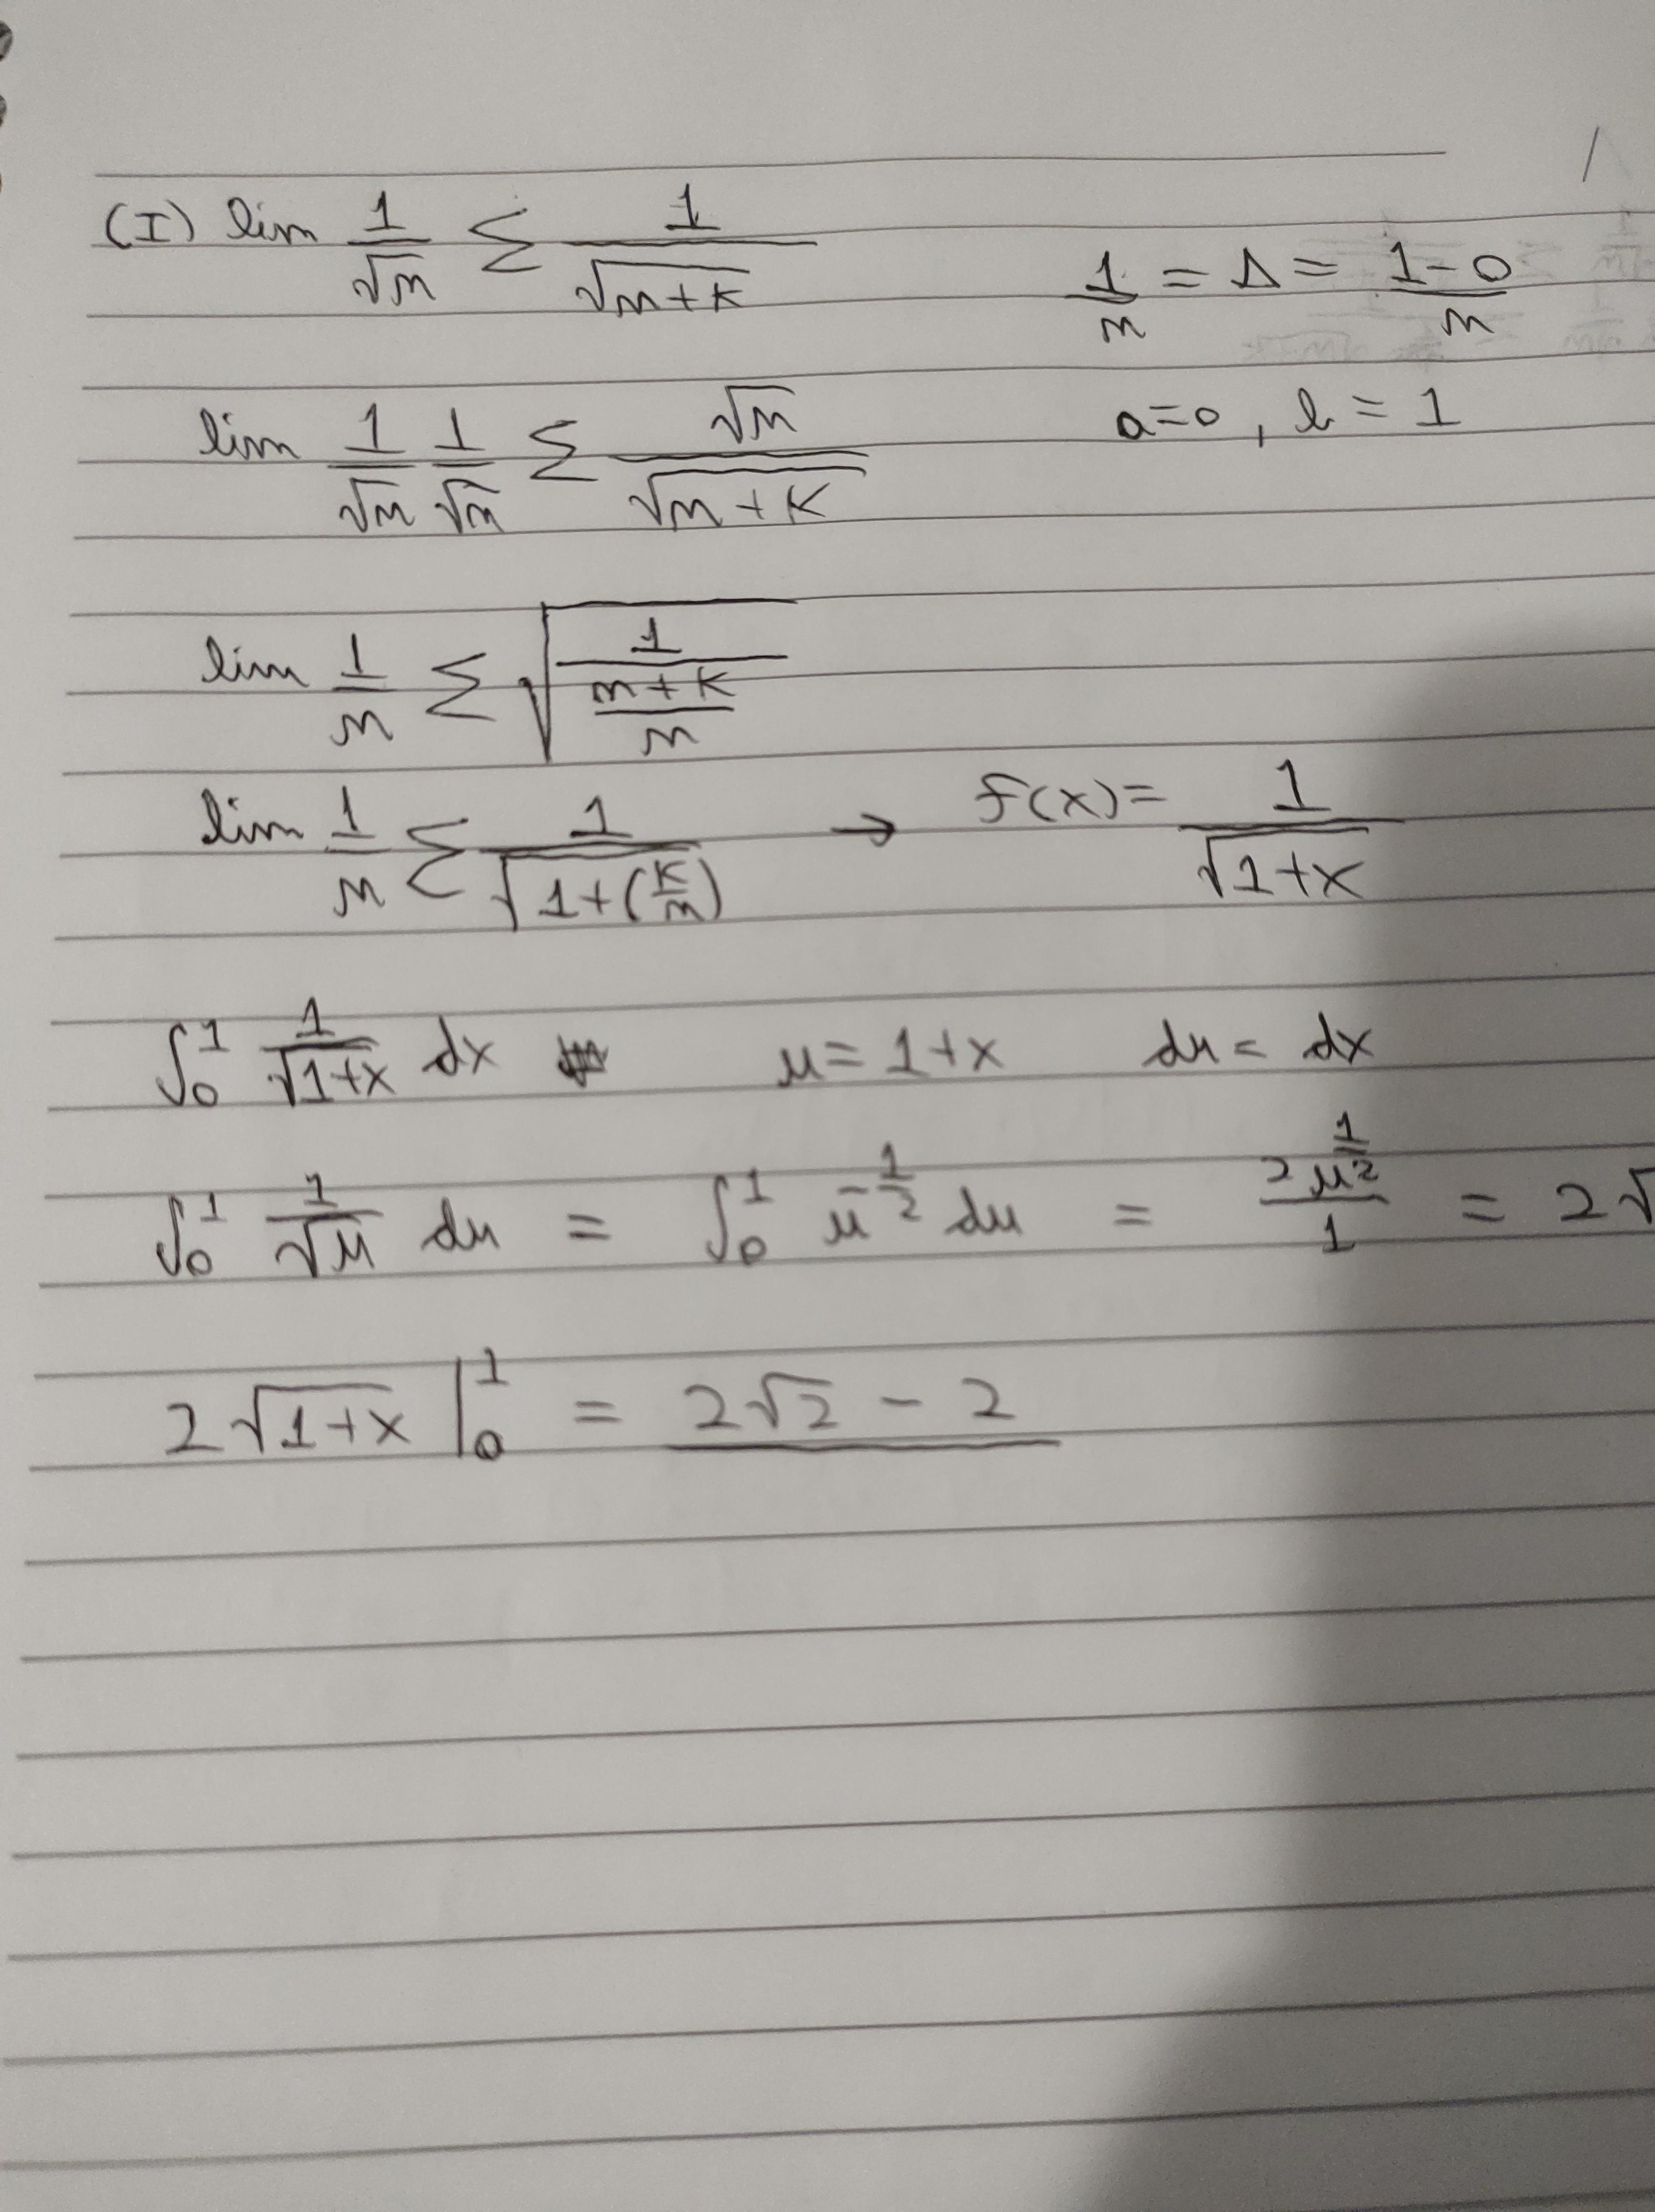
\includegraphics[scale=0.14]{q11}
\end{figure}
\begin{figure}[h!]
	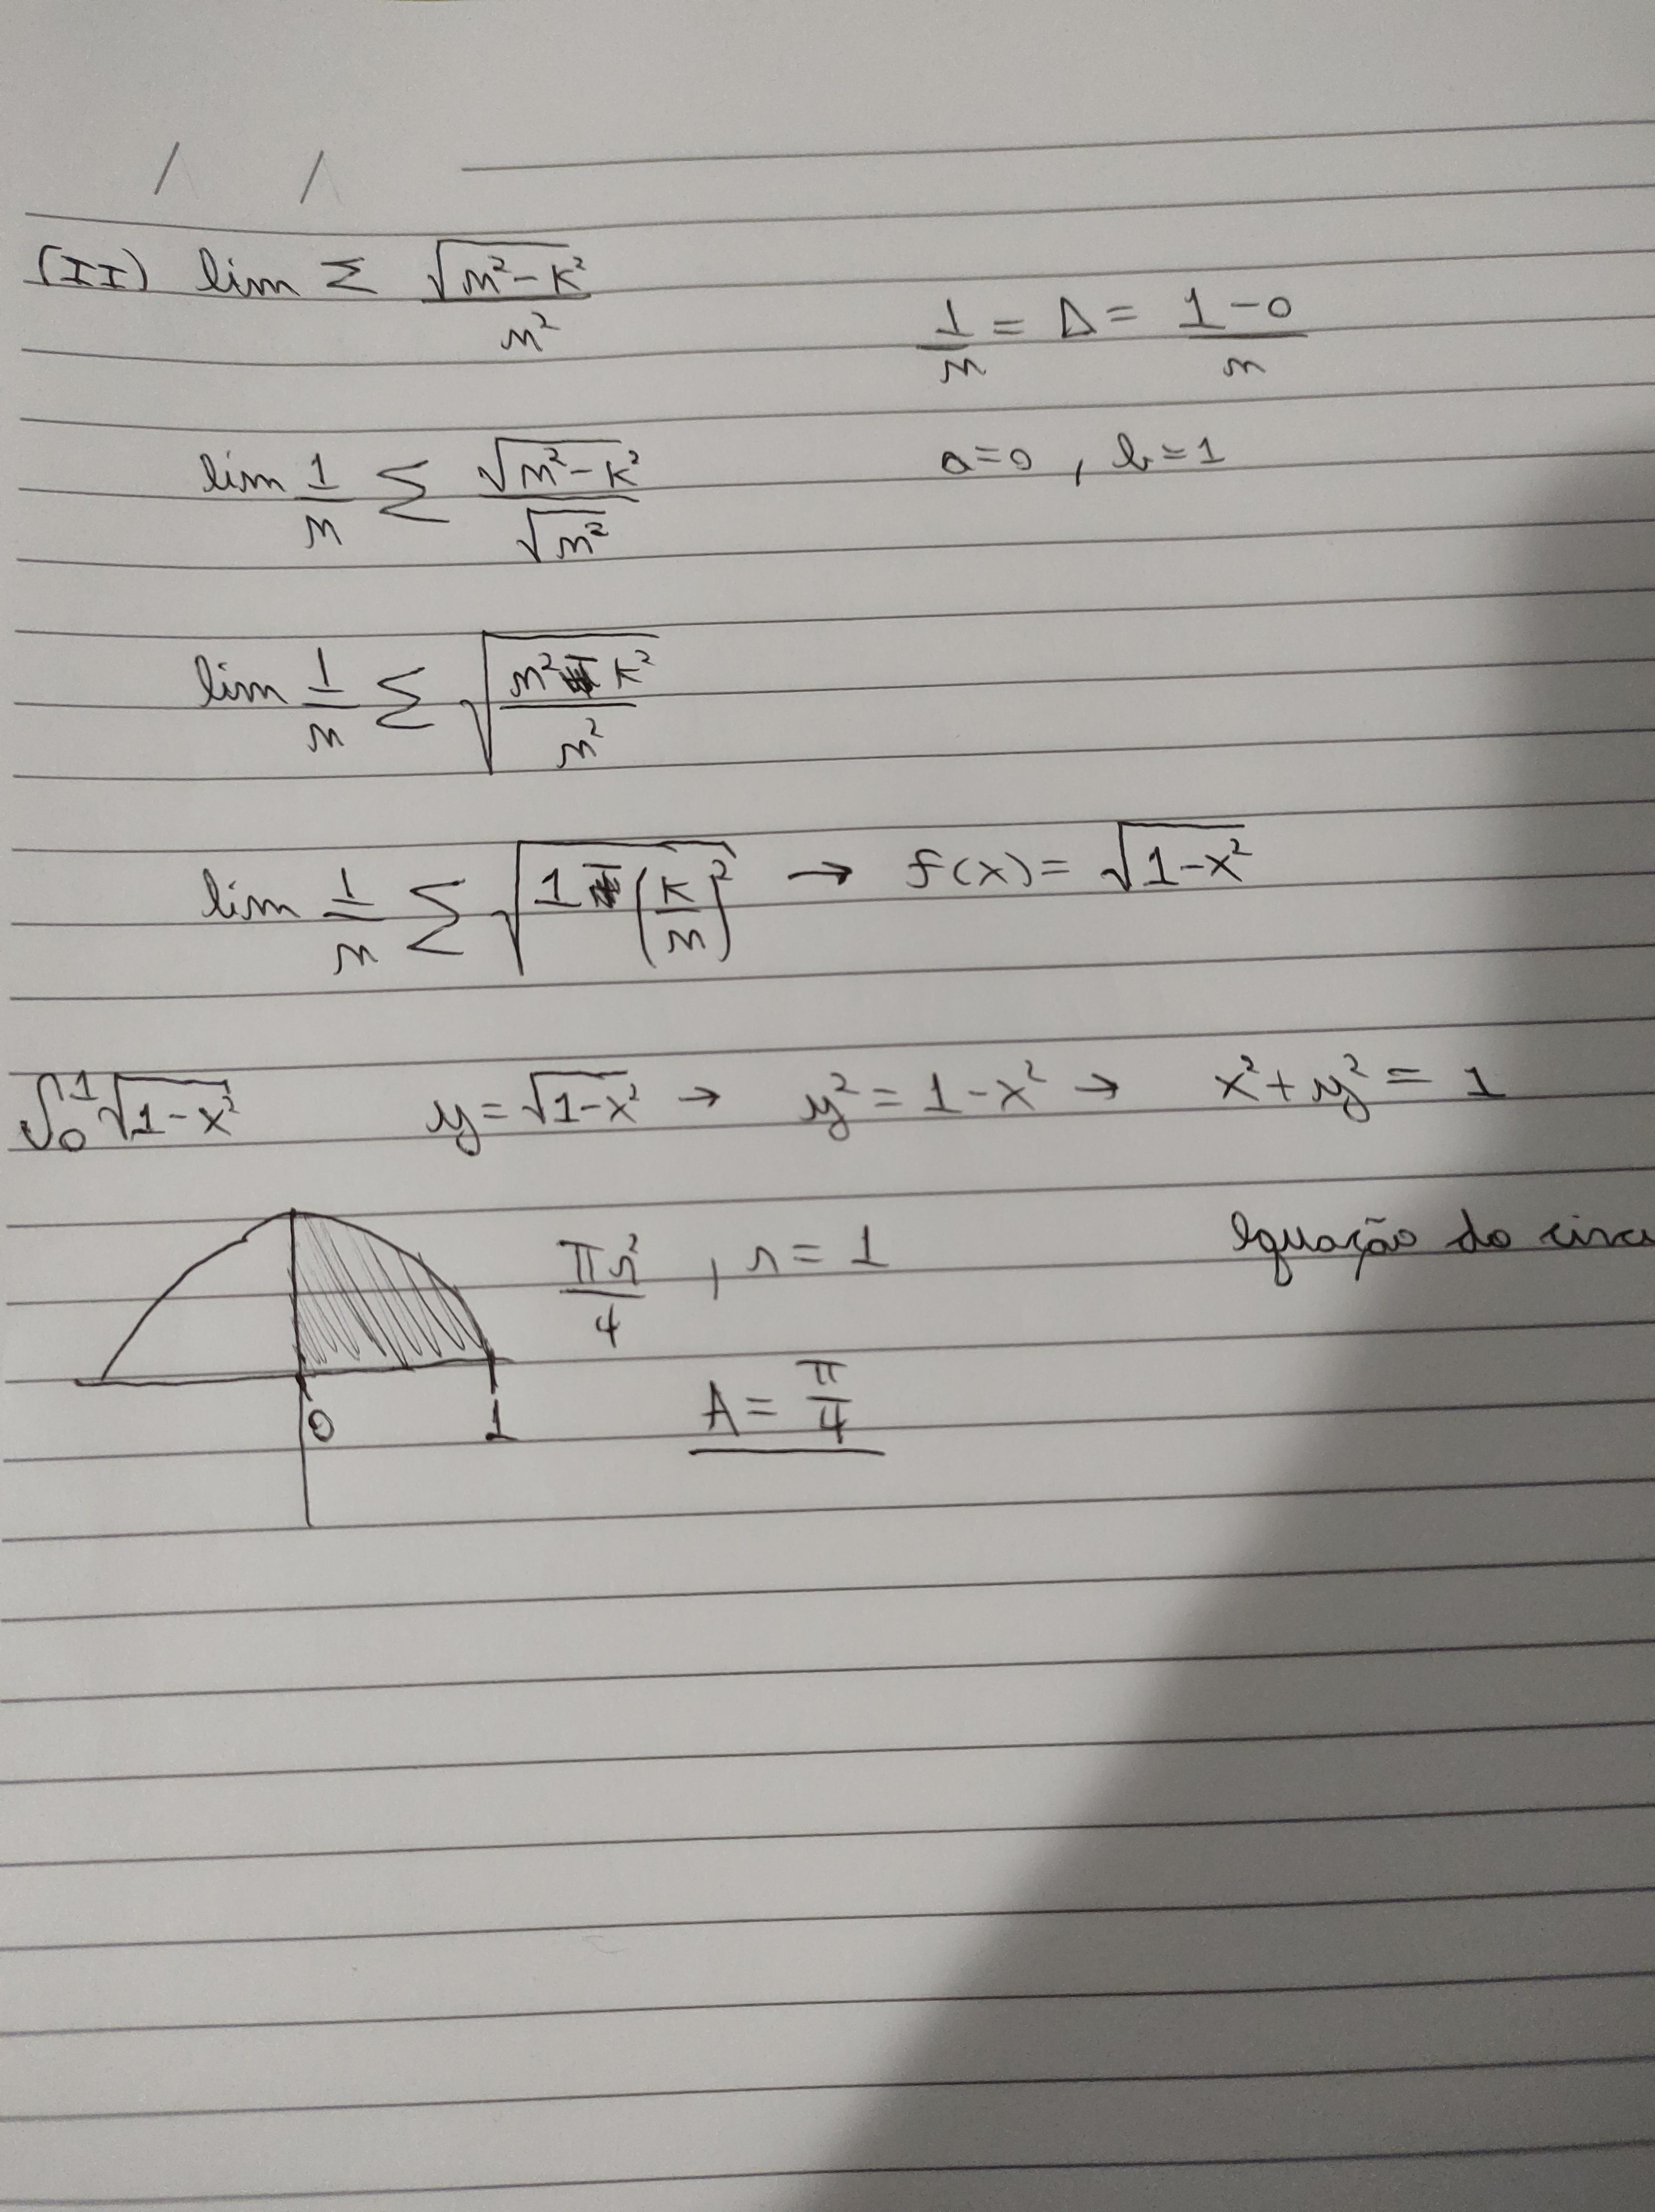
\includegraphics[scale=0.14]{q12}
\end{figure}

\begin{figure}[h!]
	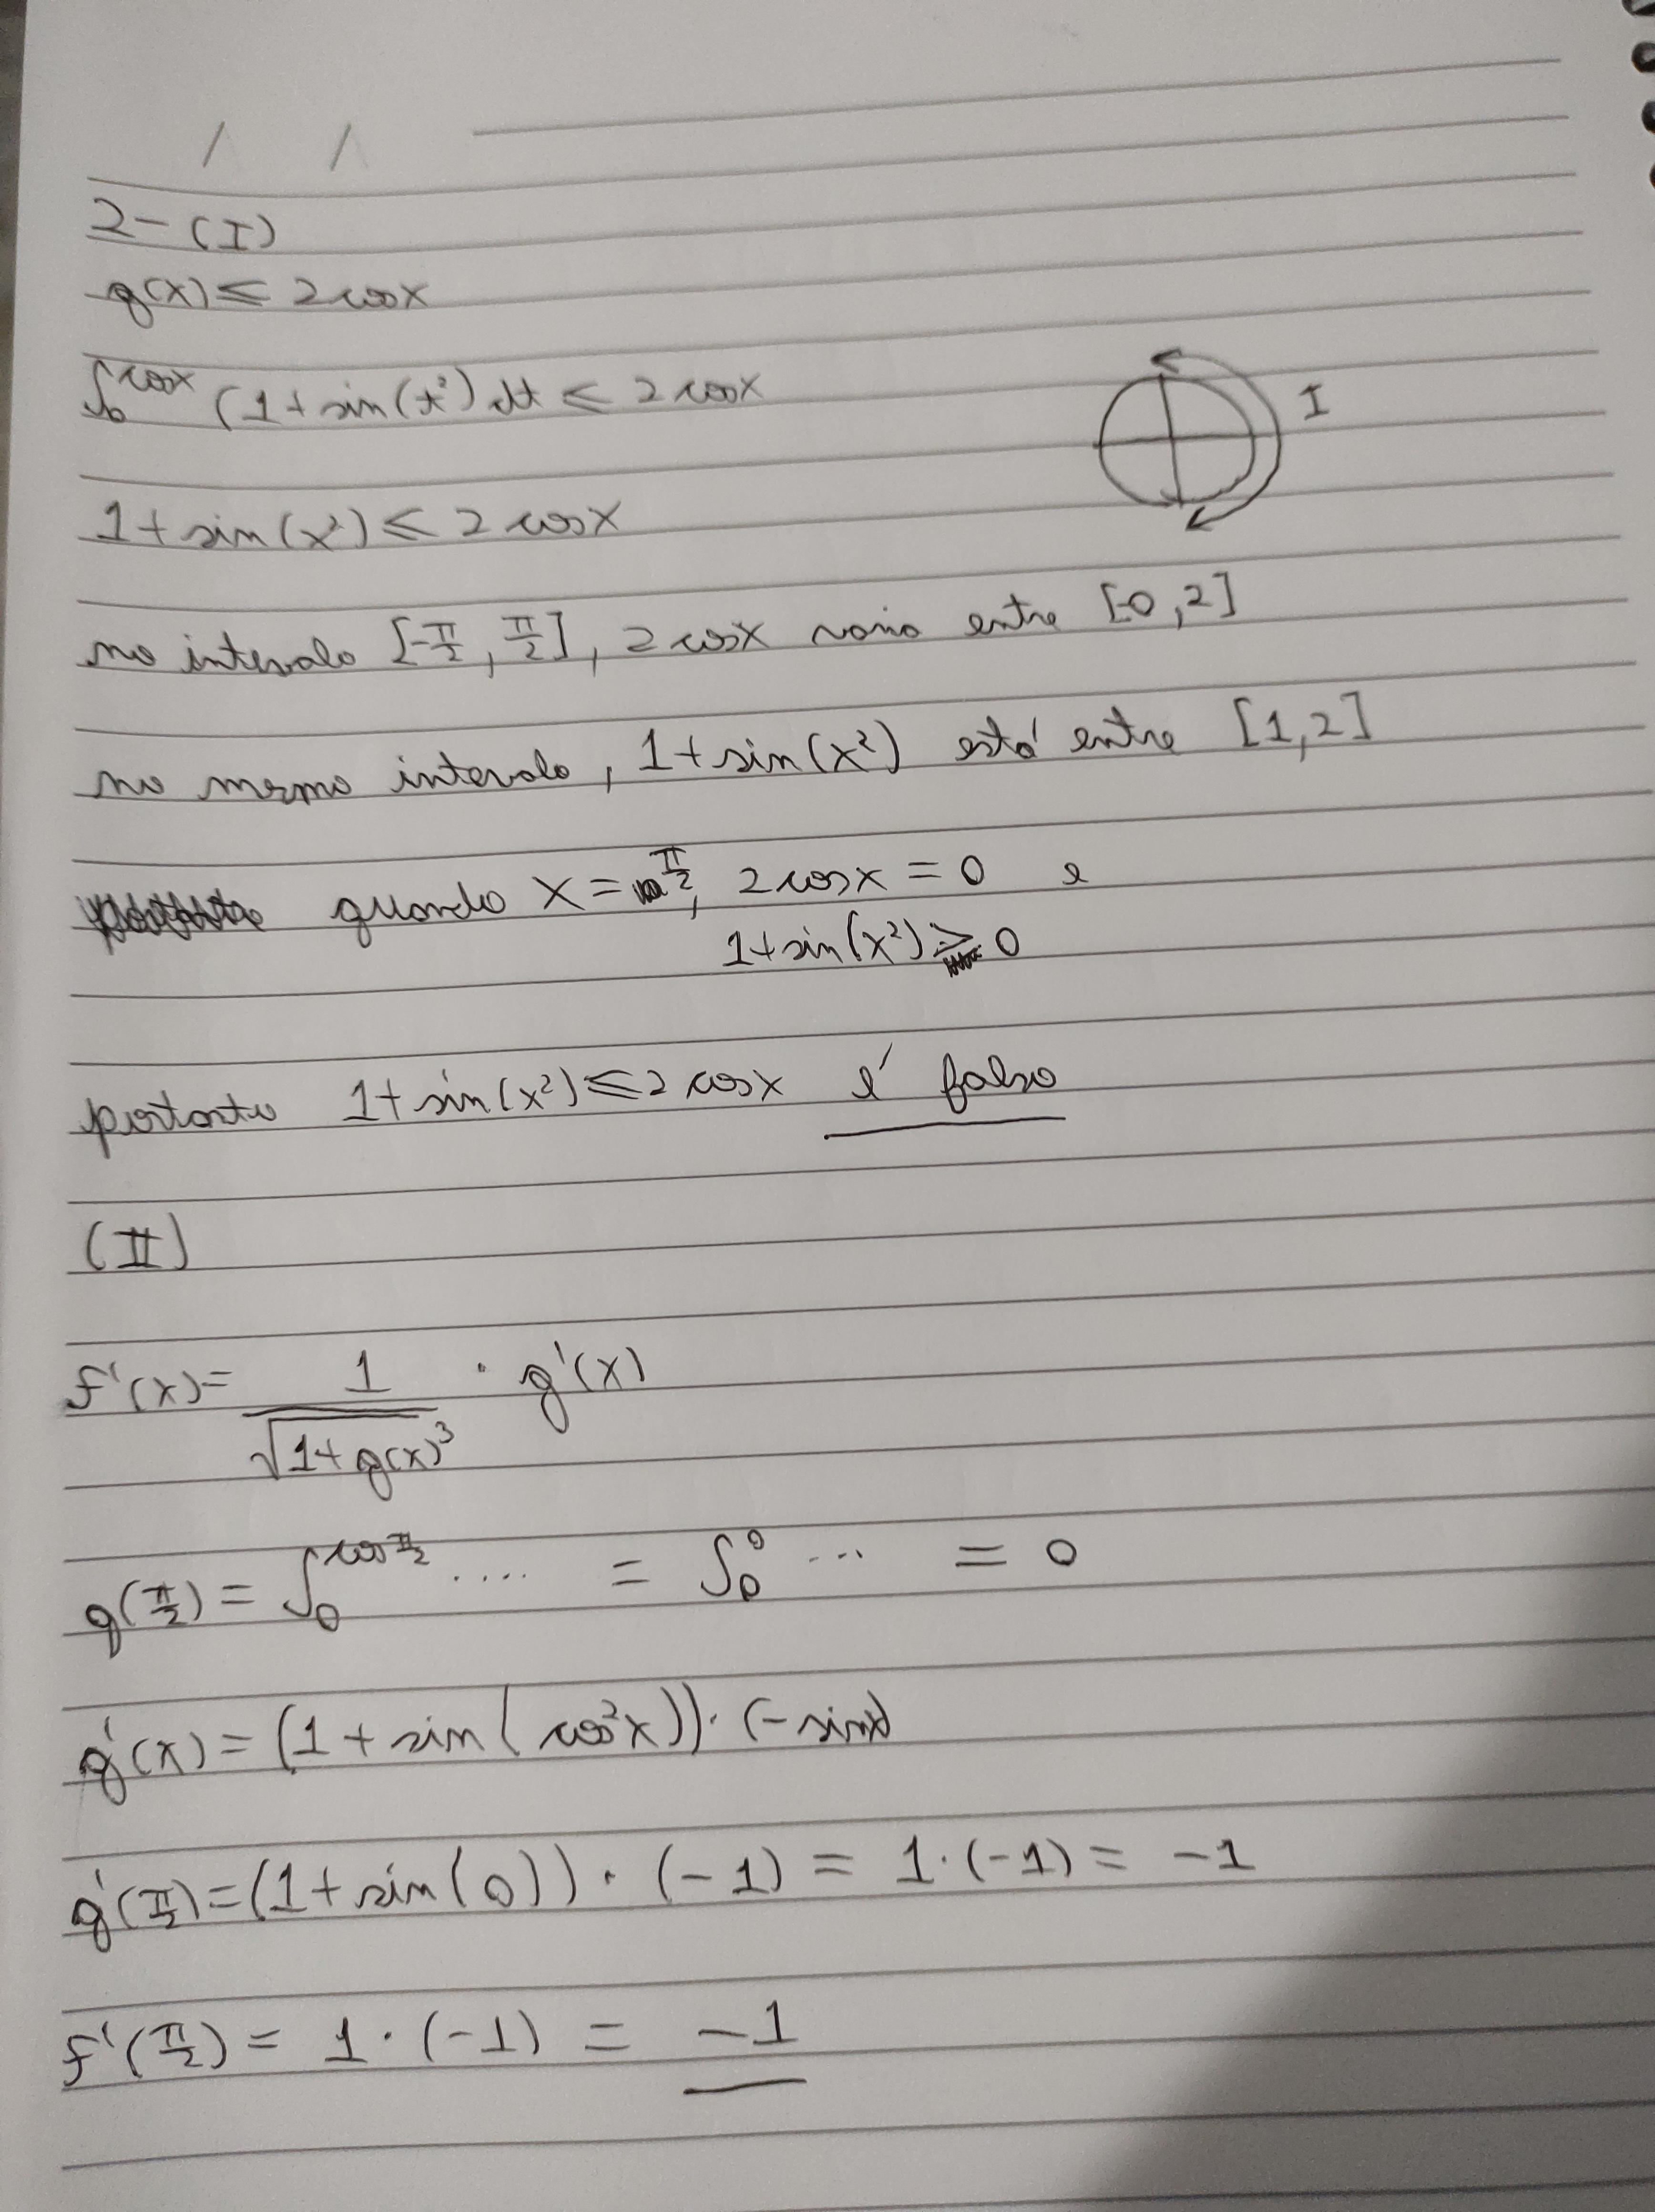
\includegraphics[scale=0.14]{q2}
\end{figure}

\begin{figure}[h!]
	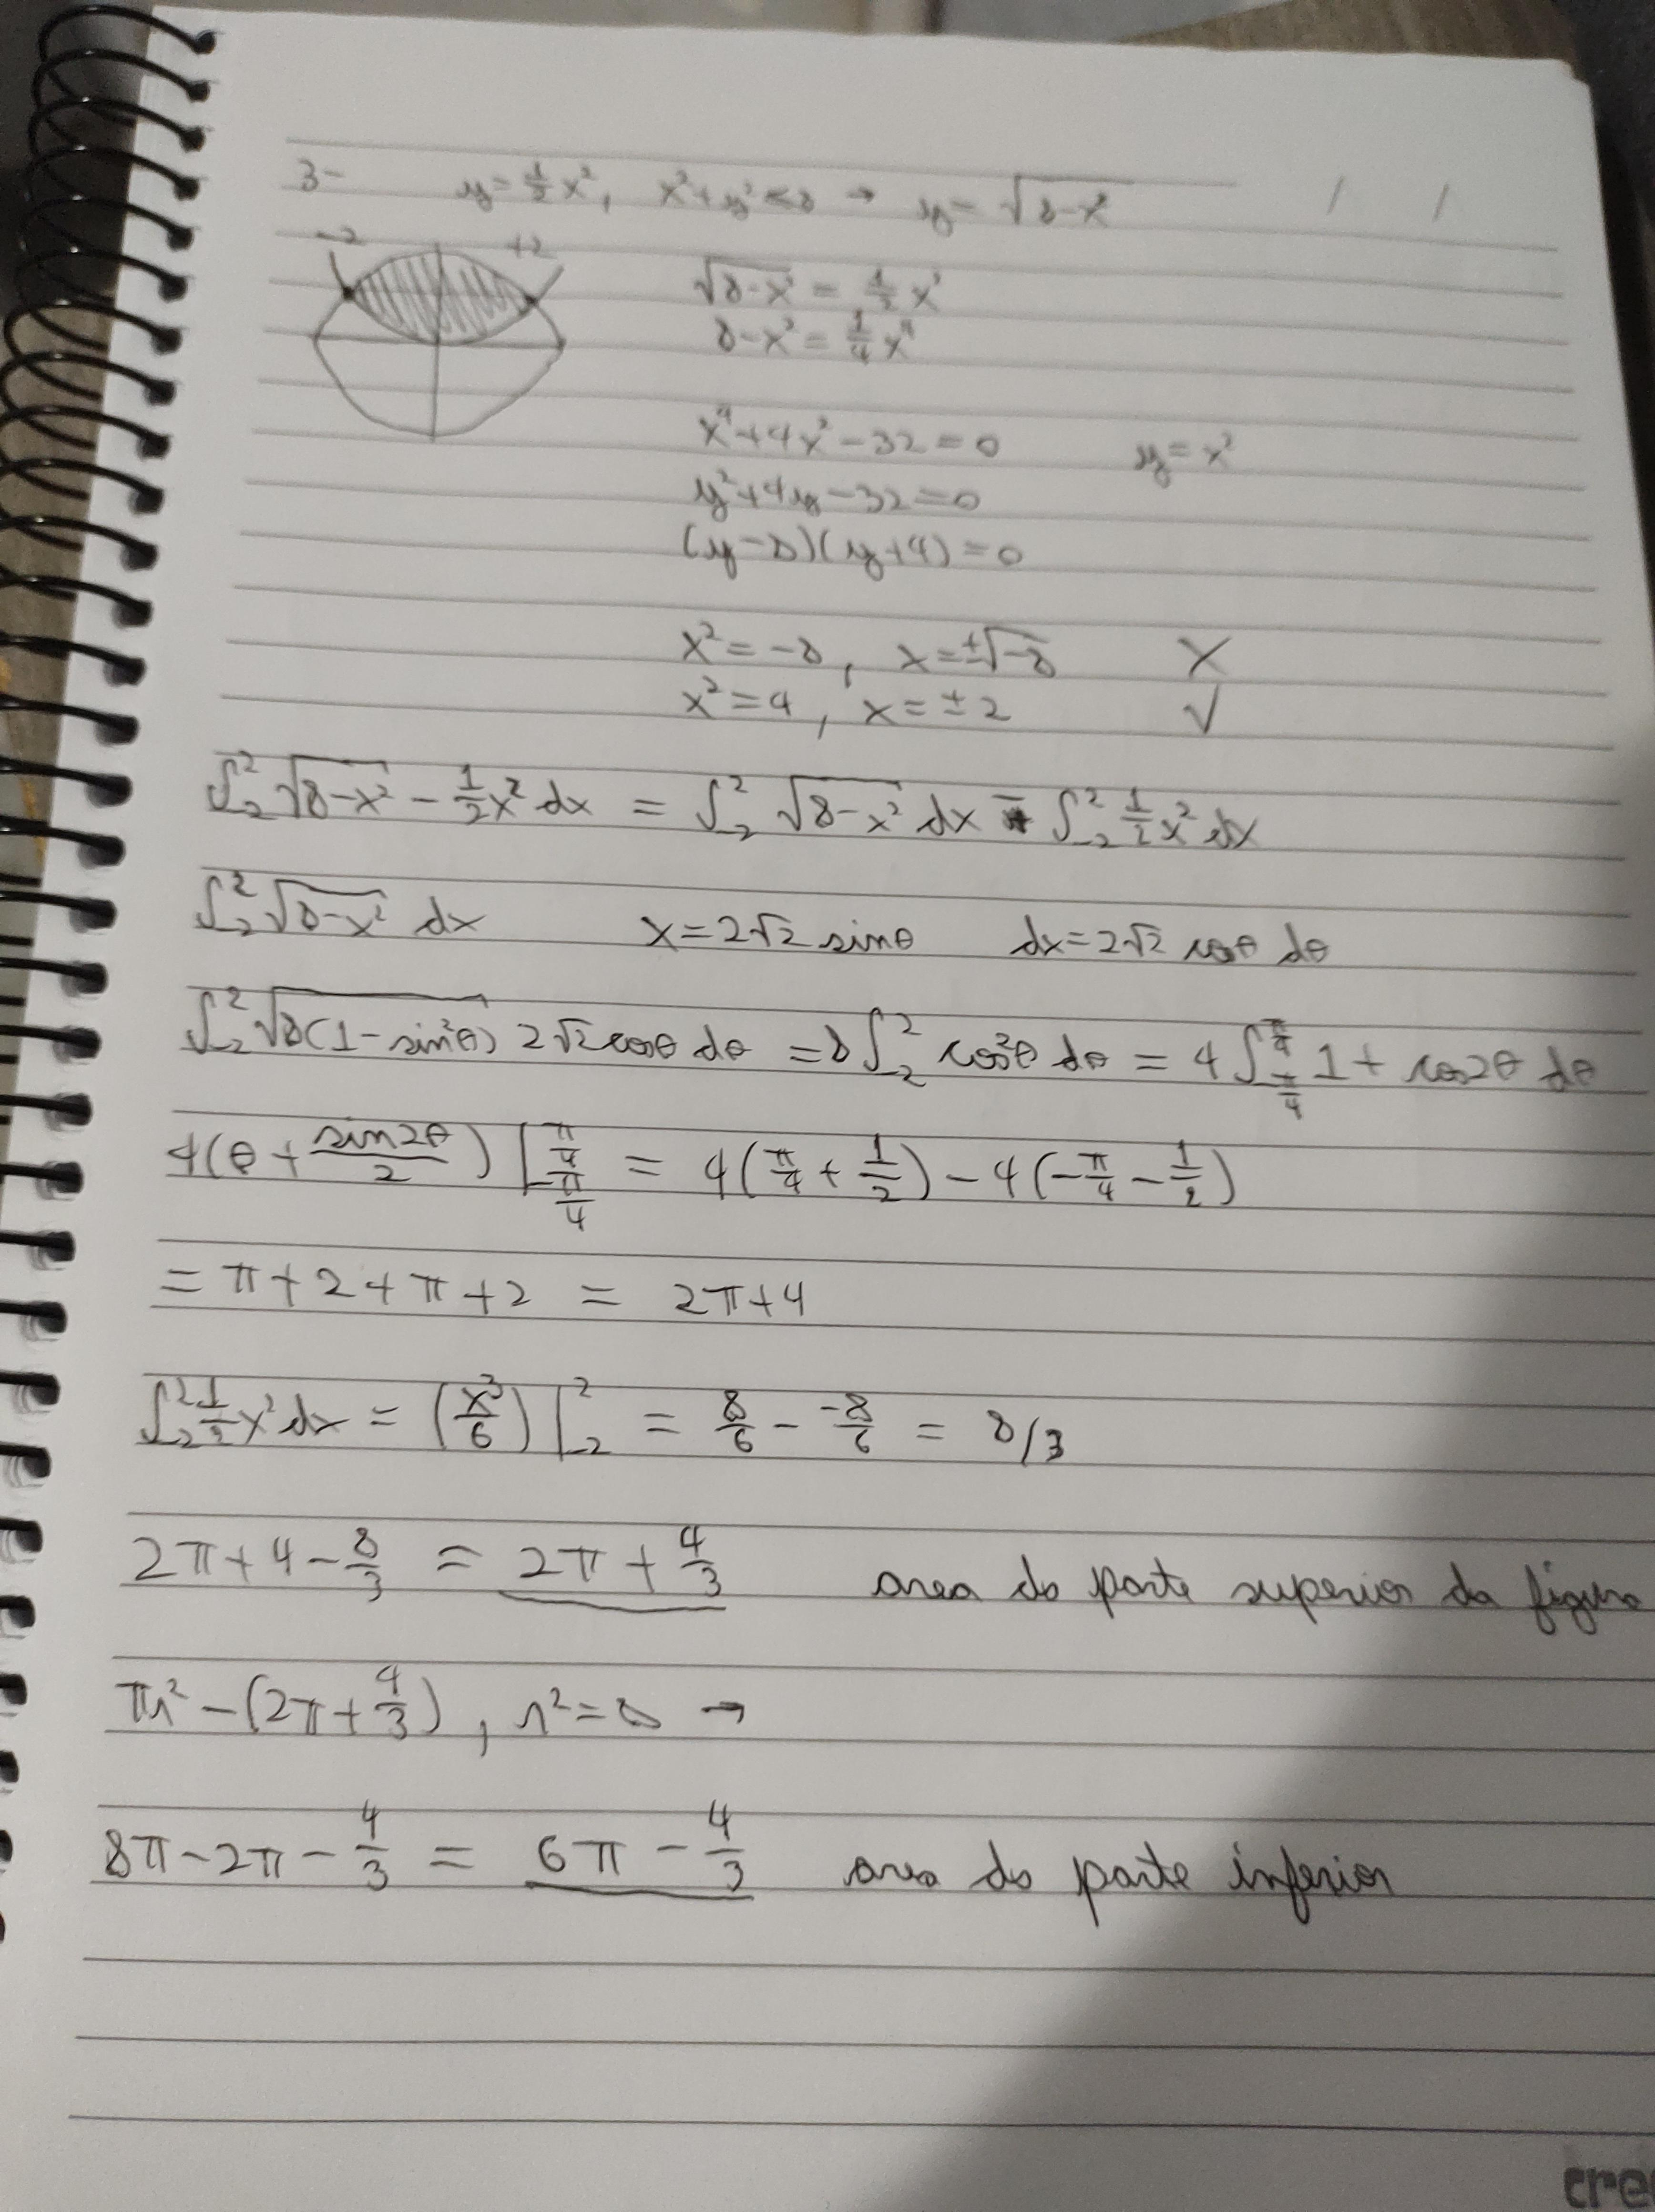
\includegraphics[scale=0.14]{q3}
\end{figure}

\begin{figure}[h!]
	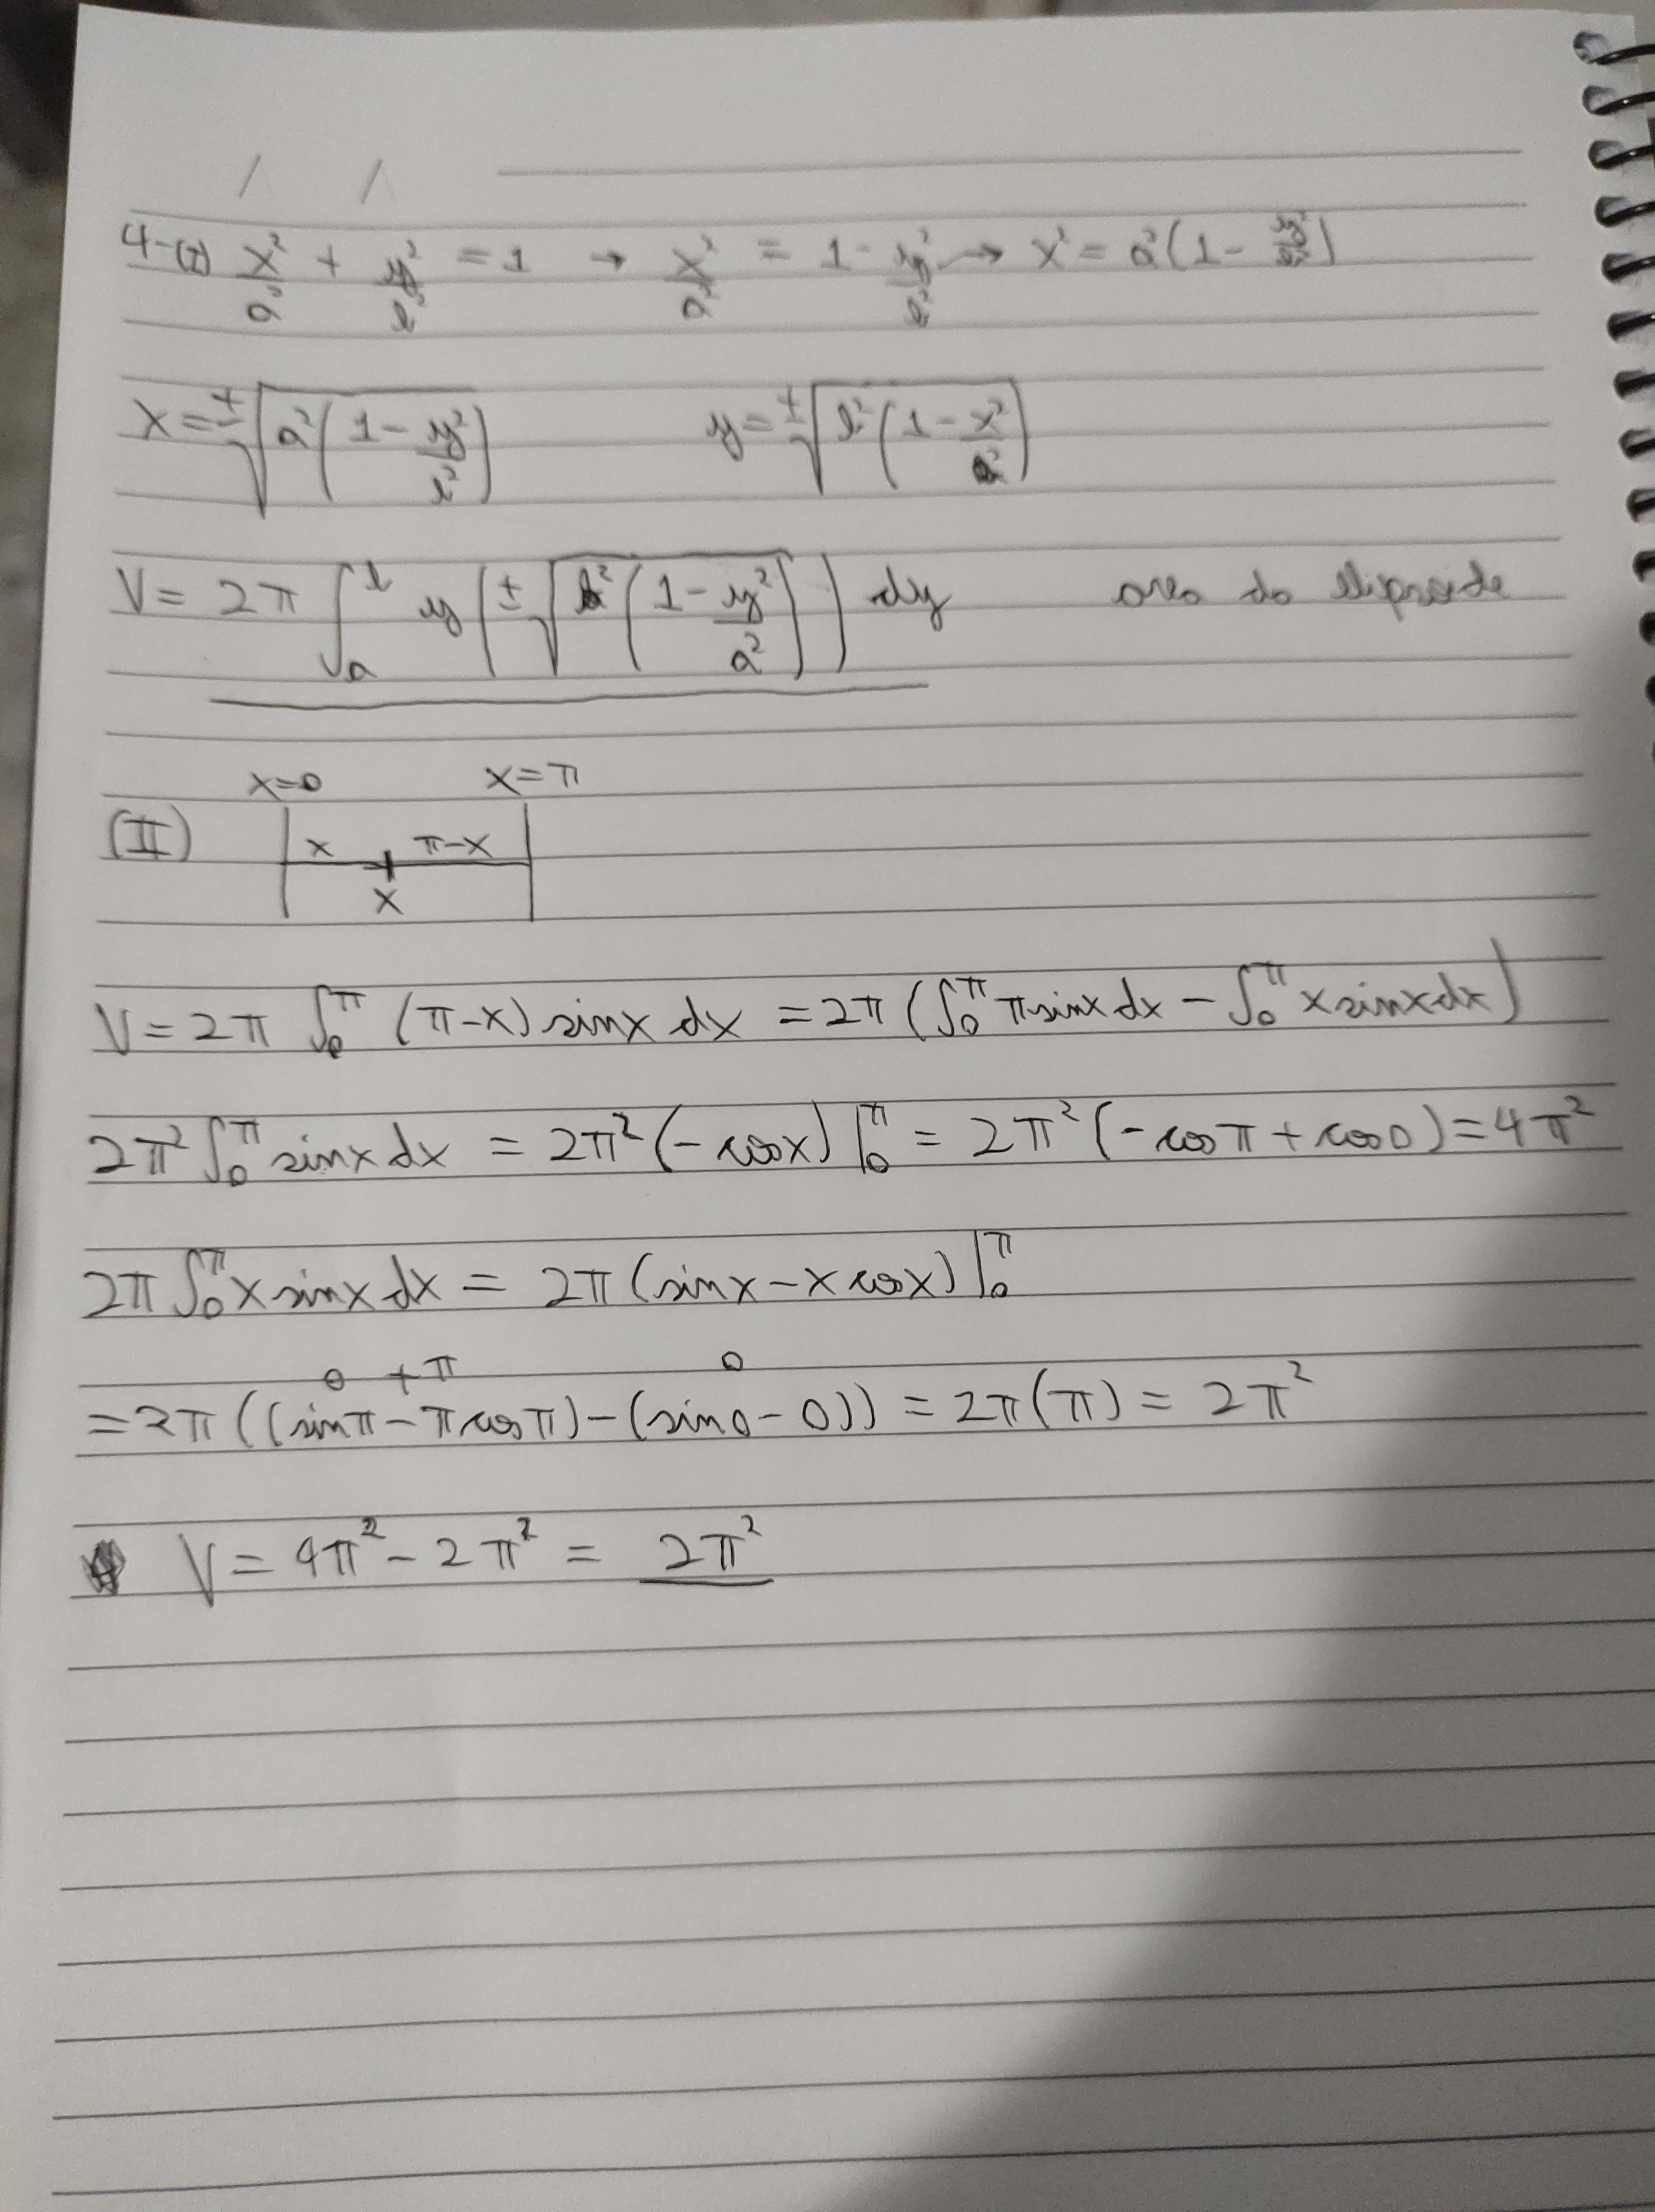
\includegraphics[scale=0.14]{q4}
\end{figure}

\begin{figure}[h!]
	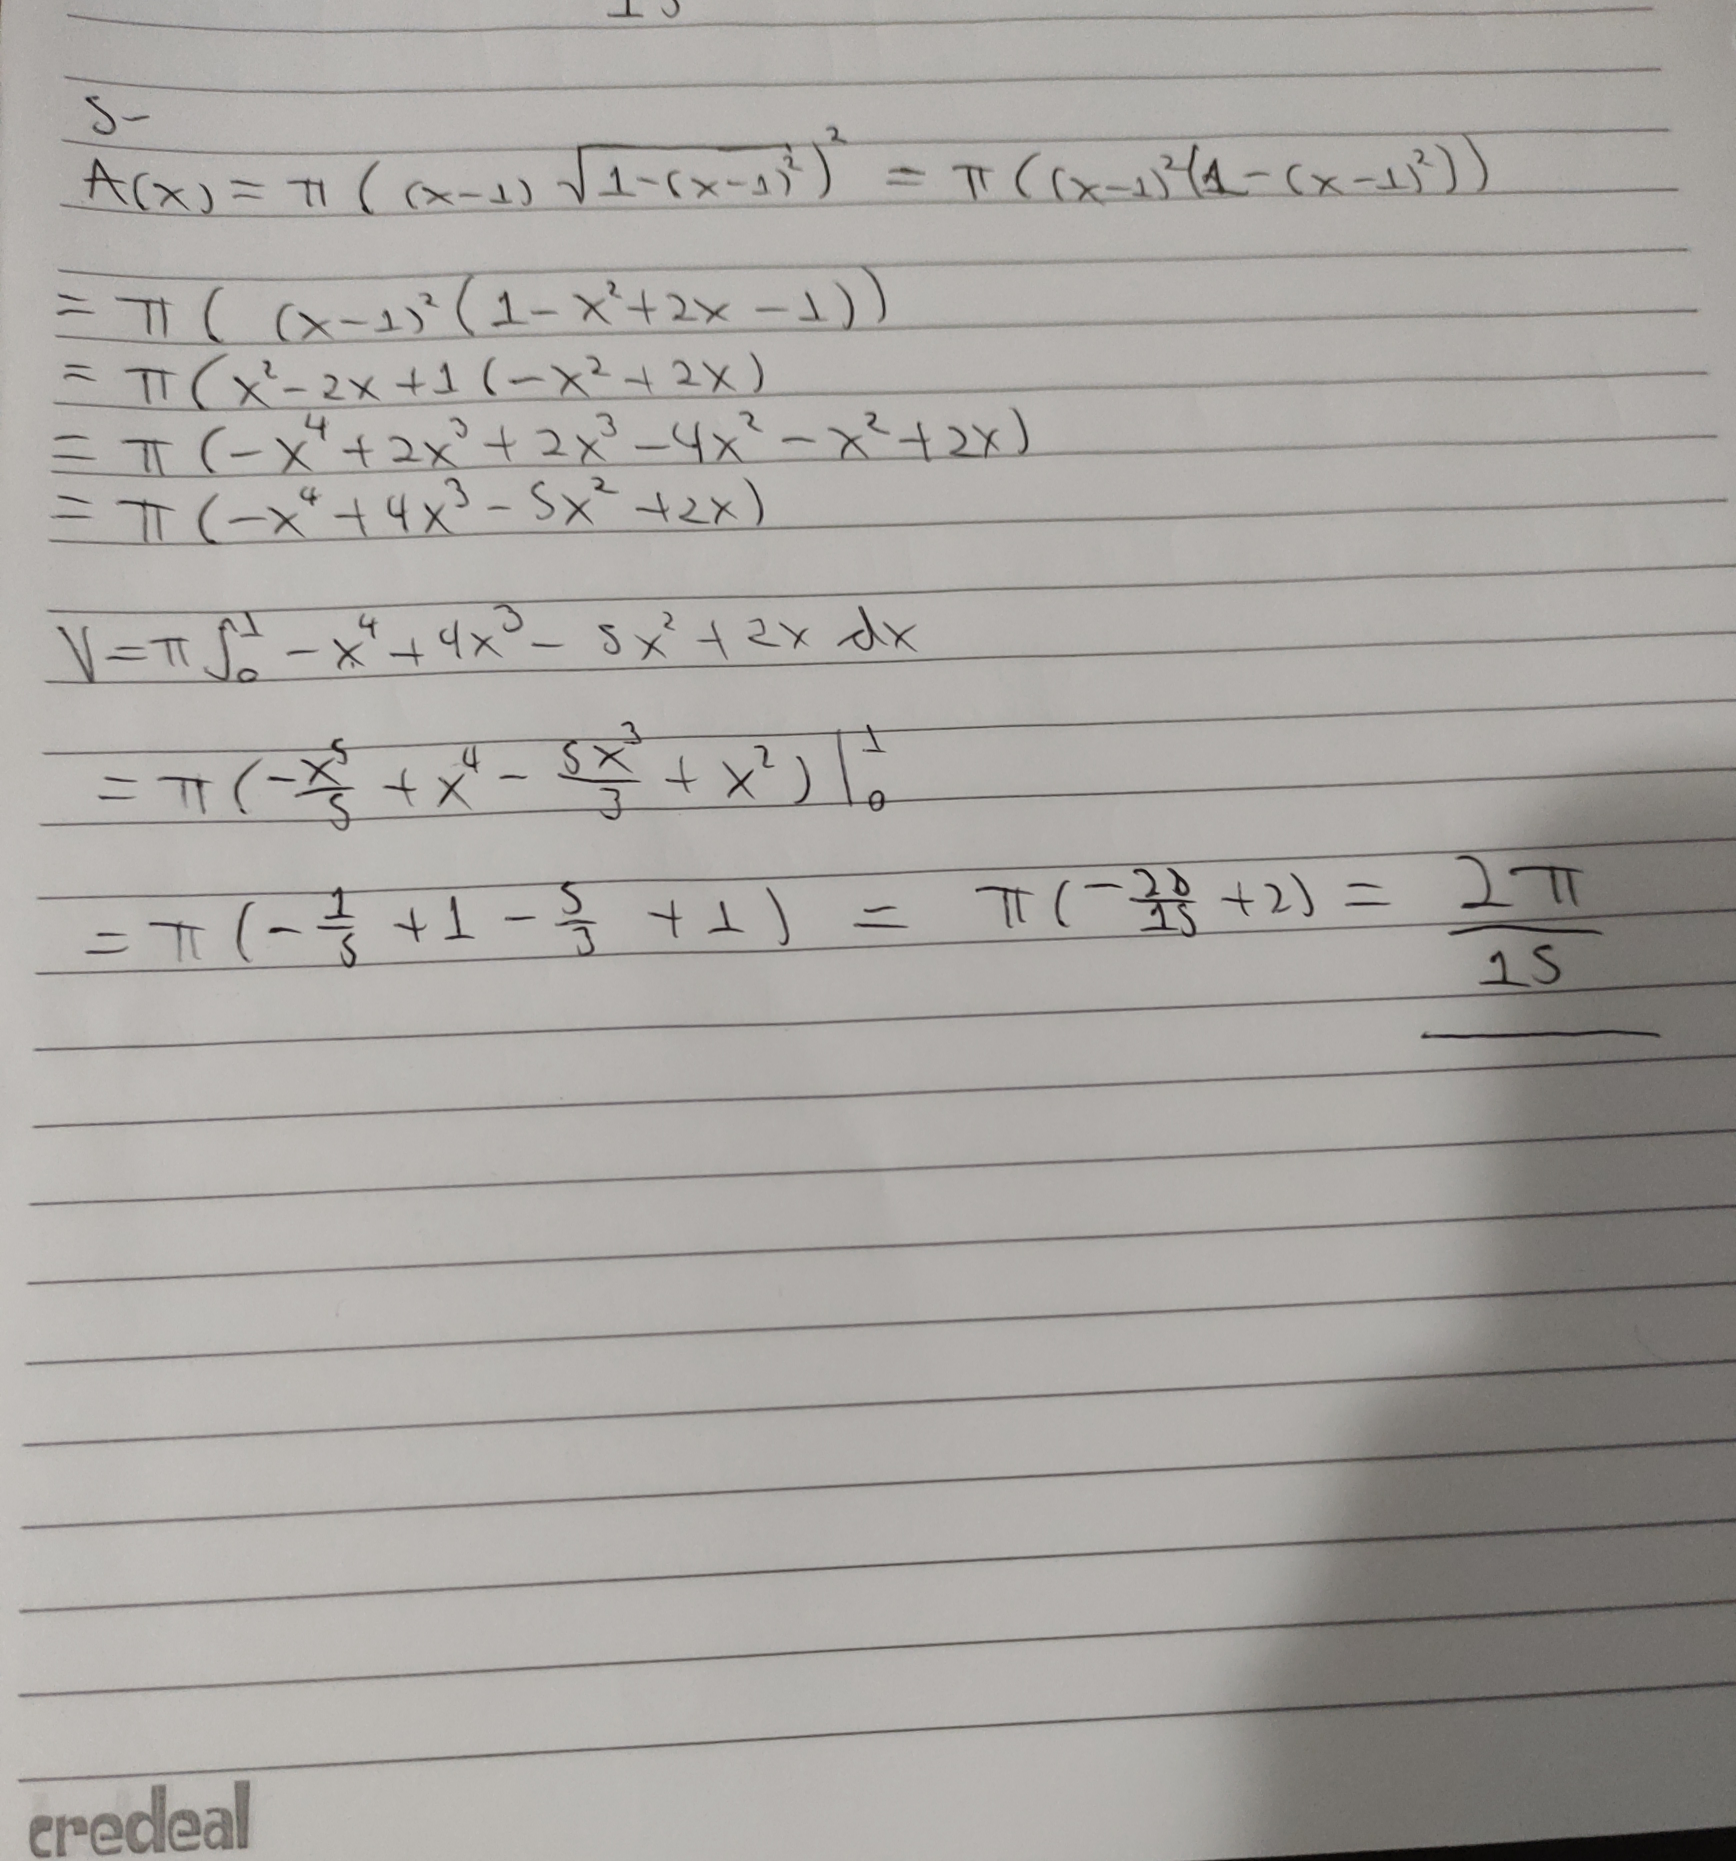
\includegraphics[scale=0.3]{q5}
\end{figure}
	

	
	
	
	
	
\end{document}